% vim: spell spelllang=en: spell: tw=0: ai: sw=2: ts=2: sts=2: lbr: noet: list:
% lcs=tab:>-,trail:-,eol:%
%% bare_conf.tex
\documentclass[a4paper,conference]{IEEEtran}
\usepackage[utf8x]{inputenc}
\usepackage[T1]{fontenc}
\usepackage{amsmath}
\usepackage{xspace}
\usepackage{microtype}
\usepackage{setspace}
\setstretch{1.05} %.971}
\usepackage{graphicx}
\usepackage[left=1.57cm,right=1.57cm,top=0.95cm,bottom=2.54cm]{geometry}
\usepackage[skip=0pt]{caption}
\graphicspath{{./svg/}{./graphs/}}
\DeclareGraphicsExtensions{.pdf,.jpeg,.png}
\usepackage{minted}
\setminted{fontsize=\scriptsize}
\setmintedinline{fontsize=\small}
\usepackage{url}
\usepackage[pdftex,hyperfootnotes=false,colorlinks=true,linkcolor=blue,citecolor=blue,urlcolor=blue,bookmarks=false]{hyperref}
% to enable \thanks command
\IEEEoverridecommandlockouts

\newcommand{\riscv}{\textsc{\small RISC-V}\xspace}
\usepackage{xcolor}

\begin{document}
\title{Challenges when Compiling for 128-bit Architectures}

% blind review
\author{\IEEEauthorblockN{~\thanks{~}}
\IEEEauthorblockA{}}


%% To uncomment for the final version
\author{\IEEEauthorblockN{Conrado~Ivan Garcia~Reyes and Frédéric Pétrot}
\IEEEauthorblockA{Univ. Grenoble Alpes, CNRS, Grenoble INP\textsuperscript{*}\thanks{\textsuperscript{*}Institute of Engineering Univ. Grenoble Alpes}, TIMA, 38000 Grenoble, France \\
\mintinline{sh}{conrado-ivan.garcia-reyes@grenoble-inp.org}, \mintinline{sh}{frederic.petrot@univ-grenoble-alpes.fr}}}

\maketitle
\thispagestyle{empty}
\pagestyle{empty}

\begin{abstract}
Although 128-bit architectures are far from being necessary today, the increase in physical and virtual address space is undoubtedly a trend on processors.
Assuming 128-bit pointers become available, the impact of this virtually infinite addressable space on the software stack will very probably be huge.
In this paper, we address the issue of compiling for such architecture, and study the changes for a compiler that can make use of such a big address space.
The architecture used to study the 128-bit compilation problem is the \riscv T-extension, which defines a 128-bit \emph{instruction set architecture}. For the compiler we choose to work with the LLVM compiler, due to its modularity and ample documentation and community.
\end{abstract}

\section{Introduction}
According to~\cite[Chapter 7]{waterman2014risc}, should today's super-computer trend continue, single address space 64-bit computers could be short of physical addresses by 2030.
Computer history has taught us that while temporary PAE-like~\cite{collins1996paging} solutions might exist for some time, the flat 128-address design will eventually emerge as the best solution.
In that situation, naturally, the general purpose registers of a processor will end up being 128-bit wide.
Clearly, not all computers will be 128-bit, and we are speaking here of a big number of machines sharing a large amount of memory, such as high-performance computing clusters.
Another advantage of a larger memory space, is the use of techniques like CHERI that allow memory pointers to hold information that could improve security in information systems. 

Making the move towards 128-bit registers and addresses is a micro-architectural and architectural challenge, given the fact that transistor technology scaling as we knew it has been over for a decade or so~\cite{mack2011fifty}.
It is also a software challenge, as the whole software stack has to be adapted and software modified with the new architecture in mind.

In this paper, we focus on an important though modest part of the software stack: the compiler.
We study in which places this change in size has notorious influence, and propose some solutions to mitigate the issues it raises.

The paper is organized as follows.
Section~\ref{sec:bg} summarizes the \riscv 128-bit specificities.
Section~\ref{sec:di} Presents our analysis of the compilation flow with the challenges at hand.
We also propose some leads to cope with these challenges.
Section~\label{sec:fp} explores problems we might encounter while migrating to a 128-bit architecture. 
Section~\ref{sec:ex} relates the experiments we made to compile code for RISCV 128 bits , and we finally conclude Section~\ref{sec:cc}.


\section{Background}
\label{sec:bg}
\subsection{Summary of the \riscv specification relevant to 128-bit}
To the best of our knowledge, the \riscv specification is the first one to introduce accurately, although informally, what could be a 128-bit processor.
It has interesting assets: it is simple; has 32 general purpose registers all of the same size; makes instructions working by default on the natural size of the processor registers (e.g. the \mintinline{asm}{add} instruction has the same opcode whether the processor has 32, 64 or 128-bit registers); naturally extends existing instructions when necessary (e.g. the shift immediate instructions have an immediate on 5, 6 or 7 bits depending on the registers size); and provides specific instructions for narrower computations (e.g. the \mintinline{asm}{w} suffixed instructions operate on 32-bit data, and the \mintinline{asm}{d} suffixed ones on 64-bit data).
Memory accesses are originally suffixed by the size of the access, so the 128-bit version simply adds the \mintinline{asm}{lq} and \mintinline{asm}{sq} instructions to access quad-words.

This specification however has also an unusual property: the size of the registers, called \mintinline{asm}{xlen} in the specification, might be run-time configurable.
The machine-mode (highest-privilege level in \riscv parlance) register size, \mintinline{asm}{MXLEN}, can be defined by setting the two upper bits of the Machine ISA (\mintinline{asm}{misa}) register.
If running a 128-bit machine, it might be set to 128, 64 or 32, and if running a 64-bit machine, it might be set to 64 or 32.
In addition, supervisor-mode and user-mode \mintinline{asm}{xlen}s (\mintinline{asm}{SXLEN} and \mintinline{asm}{UXLEN}) can also be set dynamically, by changing bitfields in the processor status register of the appropriate modes.

\section{Study of the Compilation Challenges}

\subsection{Traditional Compilers}

Since computers work with machine code that is difficult to read and write, computer scientists have been working for decades on tools to abstract away the hardware related details. Among those stand low level programming languages like C and C++, that nowadays often serve as back to languages manipulating high level concepts. As such, having efficient compilers for these language is a necessary step for anything else. The compilation process of a traditional compiler is to parse the code and validate any syntax or context errors. Then the parsed code generates assembly code that is highly optimized, and then produces machine code.

\label{sec:di}
\begin{figure}[hbtp]\center\leavevmode
	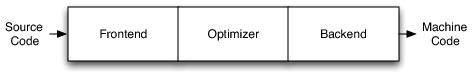
\includegraphics[width=1\linewidth]{svg/SimpleCompiler.png}
	\caption{Traditional compiler organization}
	\label{fig:llvm}
\end{figure}

\subsection{LLVM Compiler}
\label{sec:di}

The LLVM compiler is an open source project created by Chris Lattner in the university of Illinois to create an intermediary representation (IR) of a high level programming language, then this IR code can be optimized independently of the target that the compiler will generate the code for. Although other compilers like, e.g. GCC, have the same structure, we chose this compiler due to it's modularity and more modern design.
Our goal is thus to modify the current \riscv target and add a \riscv 128-bit sub target back end, since LLVM already supports the \riscv32 and \riscv64 sub targets.
Figure~\ref{fig:RetargetableCompiler} illustrates the design of a retargettable compiler such as LLVM.

\begin{figure}[hbtp]\center\leavevmode
	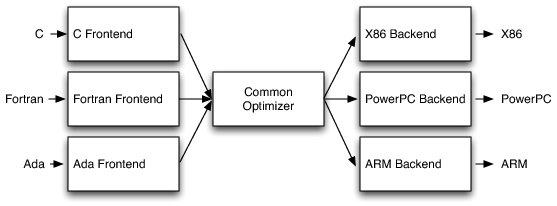
\includegraphics[width=1\linewidth]{RetargetableCompiler}
	\caption{Retargetablity of the LLVM compiler}
	\label{fig:RetargetableCompiler}
\end{figure}

The LLVM compiler pipeline is composed mainly of the front end, common optimizer, and back end. The front end determines the programming languages supported by compiler, taking care of parsing, syntax and context verification. Then the compiler generates the IR code, by selecting the IR instructions that perform the code that will be executed. These IR instructions are similar to assembly code in terms of expressiveness, but they can make use of an infinitely large register bank. Then the instructions are scheduled accordingly and the registers are allocated. This far the compiler is not different than a regular compiler, except that the generated IR code can be only executed by the LLVM compiler. Once the IR code is optimized, the compiler makes use of the selected back end that describes the target machine, including registers information, instructions available and any particularity the target may have. Then instructions are selected depending of the instructions available on the target, optimized and Assembly or machine code is generated, finally linking the generated code to an executable object. \cite{lattner2011}

The compilation process can be executed partially for any particular need regarding the compiler functionalities. 

\label{sec:di}
\begin{figure}[hbtp]\center\leavevmode
	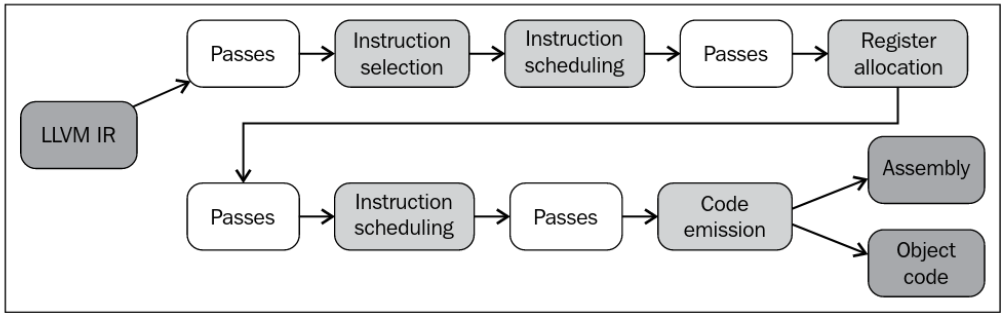
\includegraphics[width=1\linewidth]{llvmPipeline}
	\caption{Retargetablity of the llvm compiler}
	\label{fig:llvmPipeline}
\end{figure}

The objective of this paper is to identify the challenges in modifying the LLVM compiler to generate  binaries for the \riscv 128 bits T-extension, in which all the basic instructions operate on the 128 bits register size of the instruction set architecture (ISA).

As the architecture makes use of 128-bit memory addresses, pointers need to be 128-bit integers. The C programming language does already support 128-bit integers, making use of the \mintinline{c}{__uint128_t} data type. Therefore no changes on the front end are needed.

While testing the LLVM compiler, the IR code already manages to implement 128-bit data types and instructions as a single operation, therefore IR code does not need to be changed either.

Most of the work needed will be regarding the back end of the compiler, incorporating the \riscv 128-bit sub target, and any change needed regarding 128 bit memory address capabilities, as the compiler does not have support for any 128 bit architecture at the moment of writing this document.

\section{Experimentation and Lessons Learned}
\label{sec:ex}
We use the recently upstreamed 128-bit support in QEMU~\cite{portas2022fast} in order to simulate a RISCV 128-bit processor and test the ISA specifications and machine code generated by the modified LLVM compiler.

As previously stated, we made tests by generating IR code of a C language program that performs 128 bit integer operations. The generated IR code made use of 128 bit registers to perform the operations with a single instruction. 

When reading the LLVM source code and its documentations, we had to use a tool called tablegen in order to develop and maintain records of domain-specific information. This tool allowed us to write flexible descriptions and for common features of these records, being the back end target descriptions and instructions for the target.
Although the implementation for a new \riscv 128 bit subtarget is a huge development task, there is plenty of documentation regarding the LLVM compiler. 

\section{Future problems}
\label{sec:fp}
When migrating software towards a new architecture, changes are always needed, specially since the this architectural change involves memory addressing.

\subsection{Pointer size}

The biggest problem to solve is related to memory addressing, i.e. pointer size.
Although since the ANSI normalization of C in 99 assigning pointers to integer types is no longer legal without proper casting (and even though modern compiler issue warnings), supporting legacy software might prove difficult as it was when transitioning from 32 to 64-bit in the mid 90s.

Another, non-functional this time, problem that comes because of a larger pointer size is the doubling in memory consumption to perform some tasks. This problem could be solved by using memory pointer compression techniques like the ones advocated by Lattner\cite{lattner2005} in his pointer compression for linked data structures.

\subsection{Size of long sign extensions}

According to the latest ANSI C standard at the time of this writing\cite{ansiC17}:
\begin{quote}
	There are five standard signed integer types, designated as \mintinline{c}{signed char}, \mintinline{c}{short int}, \mintinline{c}{int}, \mintinline{c}{long int}, and \mintinline{c}{long long int}.
\end{quote}

Regardless of the data-type model, the standard relationship between C integral types holds true:
\begin{minted}{c}
sizeof(char) <= sizeof(short) <= sizeof(int) <= sizeof(long)
\end{minted}

In the figure Figure 4 we can observe how the data model determines the size of a pointer in relation to which data type has to be used.
We add in this table our proposal for supporting a new, 128-bit, data-model.
Although other options are possible, the one we propose fits well with large applications on general purpose core, which is the only hardware target we can think of for 128-bit processors.

Although \mintinline{c}{__int128_t} has been already defined, we need to create the long long pointer 128 bits (LLP128) standard for a 128-bit data model respecting the previous hierarchy and modifying the size of the long long value size. No literature has been found during this research regarding the LP128 or LLP128 standards.

\label{sec:di}
\begin{figure}[hbtp]\center\leavevmode
	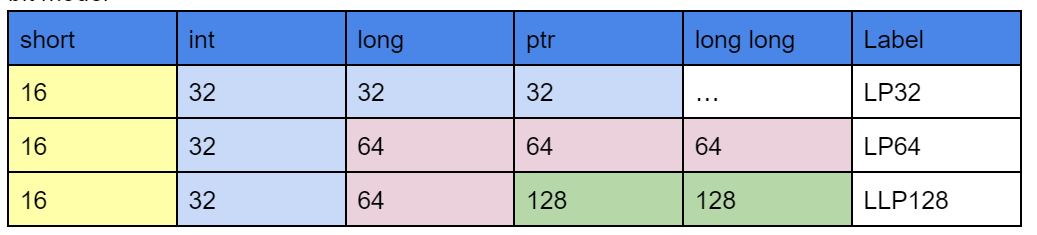
\includegraphics[width=1\linewidth]{dataModels}
	\caption{Data models differences}
	\label{fig:dataModels}
\end{figure}

\subsection{Structure packing}

Depending on the architecture, unaligned memory accesses might not be allowed, and the compiler needs to consider the padding needed for the architecture.

In a \riscv processor, unaligned memory accesses can be either done by hardware (on the high footprint implementations) or by software.
There are subtle trade-offs, in terms of performance versus memory occupancy, and the compiler shall most probably accept configuration information to take educated decisions.


\subsection{Unbalanced size of union members}

According to \cite{ansiC17}, the size of a union is sufficient to contain the largest of its members. The value of at most one of the members can be stored in a union object at any time. A pointer to a union object, suitably converted, points to each of its members (or if a member is a bit-field, then to the unit in which it resides), and vice versa.

If the pointer is changed to a different data model, the union needs to be allocated taking into consideration the size of its newest largest member in contrast to other architecture with a different data model.

\subsection{Magic numbers}

Magic numbers are the use of numerical values directly in source code, instead of the use of variables or constants. This practice can be quite problematic as magic numbers can make the code harder to read, understand and maintain. 
When magic numbers are used in order to allocate memory, it may cause problems when the software is compiled for a different architecture that doesn't have the same pointer size.  When the size allocated in memory is not enough it can cause buffer allocations and zeroing. Therefore its preferred to perform allocations using the variable size instead of a constant.

\subsection{Page size}
The \riscv architecture makes use of a 4kb page size for memory access. If the pointer size is increased to  128 bits, the capacity for the pages to store information will be reduced significantly.
Although this is not really a compiler issue, it does have an important impact on generated code performances. There are works on this topic that have been proposed, but in the context of page versus superpage allocation during compilation~\cite{magee2009case}, not on page-size aware compilation per se.
Studies to determine the proper page size and its relationship with generated code performances need to be proposed.

\subsection{Compiler optimizations}

Finally we need to study the optimizations applied by the compiler and verify if any optimization is dependent on memory address space, pointer size, or even on large integer size, since this may break particular optimization steps.

\section{Conclusion and Future Work}
\label{sec:cc}
Computer architectures with 128-bit memory addresses will be coming to a reality at some point, be it in a decade or a few of them. And while very little material is currently available, it is important to consider previous mistakes computer scientists did while migrating software during the late 90s and early 2000's, when moving from 32-bit to 64-bit.
Compiler support for the basic languages, such as C and C++, is key to a smooth transition, and benefit from the previous experience, as today type checking, also still loose for good reasons at least in C, is enforced with care in modern compilers.

Although cleared of any implementation, this paper has gone over the challenges that the 64-bit to 128-bit compilers will face, by identifying where in the compilation flow care must be taken.
There are some good news: the front-end and most of the IR can be left alone (perhaps just changing \mintinline{c}{__int128_t} introduced by GCC and adopted in LLVM) into just \mintinline{c}{int128_t}).
Most of the work will be due to memory addressing, both from the functional point of view, by working on how to handle these 128-bit pointers, and non-functional side, by taking into account effects on data-caches (instructions do not change in size or nature) and translation lookahead buffers.

It is well known that software legacy is hard to work with, even if hardware designers only dream now of building a 128-bit processor, it is time to start working or the software part to be ready in time.

\section*{Acknowledgment}
The authors would like to thank the partners of the ANR Maplurinum project and acknowledge the financial support of the French Agence Nationale de la Recherche under grant ANR-21-CE25-0016.
We are also most grateful to the QEMU and LLVM community for their help and support.
Finally we are very thankful of Campus France for allowing this student exchange, and therefore making this collaboration possible.

\bibliographystyle{IEEEtran}
\bibliography{IEEEabrv,bibliography.bib}
\end{document}
